\chapter{Herausforderungen und Probleme} % Main chapter title
\label{Probleme} % For referencing the chapter elsewhere, use \ref{Chapter1} 

%----------------------------------------------------------------------------------------
\section{RAM}

In Kapitel~\ref{Umsetzung} wurden Aufbau und Funktionsweise des Hauptspeichers und des RAM-Controllers bereits näher erläutert.
An dieser Stelle sollen nun einige Schwierigkeiten, die während der Implementierung auftraten, und die daraus resultierenden Überlegungen beschrieben werden.

\paragraph{Speicherausrichtung.} 
Ein Speicherzugriff auf $N$ Byte gilt als ausgerichtet, wenn die Startadresse dieser $N$ Byte ein ganzzahliges Vielfaches von $N$ ist~\cite[S. 96/97]{Hennessy}.
Findet z.B. ein Speicherzugriff mit der Breite von 32-Bit auf eine Adresse statt, die nicht ausgerichtet ist, die also kein ganzzahliges Vielfaches von 4 ist, ergibt sich folgendes Problem:
Nicht alle vier Byte des gesuchten Wortes befinden sich unter der gleichen (Wort-)Adresse im Speicher und können daher nicht innerhalb eines einzelnen Zugriffs erreicht werden.
Folgende Ansätze mit dieser Problematik umzugehen wurden diskutiert:
\begin{itemize}
    \item Nicht ausgerichtete Speicherzugriffe sind grundsätzlich erlaubt.
    \item Ein nicht ausgerichteter Speicherzugriff führt zu einer Prozessor-Exception, deren Handler den Zugriff korrigieren kann.
    \item Ein nicht ausgreichteter Speicherzugriff ist grundsätzlich nicht möglich.
\end{itemize}

Die Lösungsansätze eins und zwei führen unweigerlich zu Performanceeinbußen, da sie nicht in der gleichen Zeit wie ein ausgerichteter Speicherzugriff abgearbeitet werden können.
Außerdem wird in der RISC-V-Spezifikation nur für ausgerichtete Zugriffe Atomarität garantiert, wohingegen bei unausgerichteten Zugriffen zusätzliche Vorkehrungen zu treffen sind~\cite[S. 18]{RISC}.
Der vorliegende RAM-Controller wurde mit dem dritten Lösungsansatz implementiert, mit dem Vorteil, dass alle Maschinenbefehle die gleiche Zeit zur Ausführung benötigen.
Ein nicht ausgerichteter Speicherzugriff wird hier also unterbunden, d.h. der Maschinenbefehl wird ignoriert und hat keinerlei Auswirkung.

Umgesetzt wurde dies wie folgt:\\
Bei einem nicht ausgerichteten Schreibzugriff wird der Schreibvorgang nicht unterbrochen, allerdings wird in die jeweilige Speicherstelle einfach der ürsprünglich dort enthaltene Wert zurückgeschrieben.
Somit wird der Speicher nicht verändert.\\
Wird dagegen lesend auf eine nicht ausgerichtete Adresse zugegriffen, sendet der RAM-Controller über seinen \textit{dsbl\_wr\_reg}-Port ein Signal an den Dekodierer, der diese Information (\textit{en\_write = false}) an die Registerbank weiterleitet und somit einen Schreibzugriff auf das Register unterbindet, in das der zu lesende Wert aus dem RAM ursprünglich geschrieben werden sollte.

\paragraph{Schreibprozess.} 
Da auf den Hauptspeicher nur ein 32-Bit breiter Zugriff möglich ist, muss der RAM-Controler vor einem Schreibzugriff der Breite 8- oder 16-Bit die adressierte Speicherstelle lesen um diese verändern und anschließend zurückschreiben zu können~(\ref{subsec:RAM}).
Herausforderung bei der Umsetzung dieser Maschineninstruktionen war es, diese in zwei Takten durchführen zu können, um die Anzahl der Takte pro Instruktion nicht erhöhen zu müssen.
Abbildung~\ref{fig:write} zeigt beispielhaft, wie ein Schreibprozess in den RAM durchgeführt wird.
Links sieht man die Namen der enstprechenden Ports und Signale, während rechts deren Werte zum jeweiligen Zeitpunkt (siehe Taktsignal \textit{s\_clk}) dargestellt sind.

\begin{figure}[htpb]
    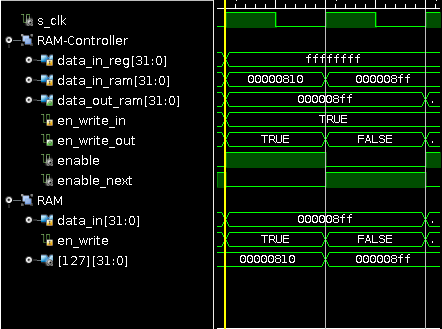
\includegraphics[width=\textwidth]{Figures/write.png}
    \caption{Umsetzung eines Schreibzugriffs in den Speicher}
    \label{fig:write}
\end{figure}

In diesem Beispiel soll ein Byte in den Speicher geschrieben werden:\\
Der RAM-Controller erhält ein Wort von der Registerbank (\textit{data\_in\_reg}), dessen niederwertigstes Byte in den Speicher geschrieben werden soll (in diesem Fall wiederum an die Position des niederwertigsten Bytes).
Gleichzeitig liest er den Wert aus der Speicherstelle, die adressiert wird  (\textit{data\_in\_ram}), um diese mit dem Registerwert zu modifizieren und in den Speicher zurückzuschreiben (\textit{data\_out\_ram}).
Vom Dekoder erhält der RAM-Controller die Information, dass ein Schreibzugriff auf den RAM erforderlich ist (\textit{en\_write\_in}), welche er direkt an den RAM weiterleitet (\textit{en\_write\_out}).
Dieser erhält den Schreibbefehl (\textit{en\_write}) allerdings kurz nach einer steigenden Taktflanke (siehe \textit{s\_clk}), weswegen der eigentliche Schreibvorgang erst im zweiten Takt erfolgt.
Um einen weiteren Schreibzugriff im nächsten Takt zu verhindern, setzt der RAM-Controller das \textit{en\_write\_out}-Signal  mit Hilfe zweier toggelnder Signale (\textit{enable} und \textit{enable\_next}) auf \textit{FALSE}.
\section{Laden von ELF-Dateien}
Es wurde versucht ausführbare C-Programme im Executable and
Linkable Format (ELF) in den Hauptspeicher (RAM) zu laden. Hierzu wurde
eine ausführbare Datei, die der
RISC-V-GCC\footnote{https://github.com/riscv/riscv-gnu-toolchain
(08.03.2017)} kompiliert hat, in den RAM geladen. Durch verschiedene
Anpassungen wurde versucht an die Stelle in der ELF-Datei zu
„springen“, die den Start der ausführbaren Instruktionen darstellen.
Der „Entry-Point“ des Programms wurde mit dem Programm \code{readelf}
ermittelt. Das Springen an diese Adresse war jedoch erfolglos, da der
Vorgang des Ladens von ELF-Dateien falsch verstanden wurde. 

%% TODO ist das so okay?!
\paragraph{Erkenntnis.} Ein ELF-Loader wäre benötigt worden, der die Datei (Instruktionen,
Variablen) an den richtigen Stellen in den Speicher läd. Loader sind 
in der Regel Teil eines Betriebssystems. Aus Zeitgründen konnte dieser
nicht umgesetzt werden, besonders weil keine Ausführungsumgebung
(Betriebssystem) für die Entwicklung der RISC-V-CPU zur Verfügung stand.
